\section{Introduction}
WASM (or WebAssembly) is an open standard binary code format close to assembly. Its initial objective is to provide an alternative to java-script and better performance in the current web ecosystems. Benefiting from its platform independence, front-end flexibility (can be compiled from the majority of languages including C, C++, assembly script, rust, etc.), good isolated runtime and speed that is close to native binary, its usage starts to arise in the distributed cloud and edge computing. Recently it has become a popular binary format for users to run customized functions on AWS Lambda, Open Yurt, AZURE, etc.

As with the technology of WASM runtime for cloud and edge computing shifts, security and privacy \cite{ pearson2009taking} issues emerge in scenarios that demand trustless \cite{wood2016trustless, chang2002trustless} computation and privacy computing \cite{xiao2012security,takabi2010security}. For instance, suppose that there is a voting hub hosted in the cloud to collect votes for proposals. The role of this service is to report the voting results to users while not leaking any information about any voters' choices. In this scenario, we would like a service that does not only provides the voting results but also provides proof to convince users that the provided results are calculated with predefined protocols (voting protocols). However since the service can not leak voters' personal choices, it should not reveal any voting ticket that is signed by a voter which makes it tricky to make the proof. 

Traditional ways to achieve trustlessness and privacy usually involve invasive changes to the source code of the service running on the cloud and those changes are usually applied in a case-by-case manner. In this work, instead of changing the code itself, we propose a novel approach by implementing \zkwasm, which is a WASM virtual machine that not only runs the WASM bytecode but also provides a zero-knowledge proof which is used to convince a verifier that the execution result is trustworthy.

The idea of \zkwasm\, is derived from ZKSNARK (Zero-Knowledge Succinct Non-Interactive Argument of Knowledge) which is a combination of SNARG (Succinct non-interactive arguments) and zero-knowledge proof. In general, the adoption of ZKSNARK usually requires implementing a program in arithmetic circuits (see Section \ref{chp:arith-circuits}) which forms a barrier for existing programs to leverage the power of it. Thus in this paper, we write the whole WASM virtual machine in ZKSNARK circuits so that existing WASM applications can benefit from ZKSNARK by simply running on the \zkwasm\, without any modification. Therefore, the cloud service provider can prove to any user that the computation result is computed honestly and no private information is leaked.

\smallskip\noindent\textbf{The Problem.}
To implement a ZKSNARK backed WASM virtual machine, we need to connect the implementation of WASM runtime with the proof system of ZKSNARK. In general, a ZKSNARK system is represented in arithmetic circuits (see Section \ref{chp:arith-circuits}) with polynomial constraints. Therefore we need to abstract the full imperative logic of a WASM virtual machine systematically and rewrite it into arithmetic circuits with constraints. Given two outputs, one is generated by emulating the WASM bytecode in WASM runtime that enforces the semantic of WASM specification, and the other satisfies the constraints imposed on the arithmetic circuits. If the circuits we write preserve the semantics, then these two outputs must be the same. Thus the proof of the ZKSNARKS derived from the circuits also shows that the output is valid as a result of emulating the bytecode in WASM runtime. 

\smallskip\noindent\textbf{Our Contribution.}
In this paper we systematically abstract the WASM runtime implementation and rewrite it into arithmetic circuits with constraints. By doing so, we have proposed and implemented the first zk-WASM virtual machine that supports WebAssembly specification. Moreover, by providing \zkwasm\, existing program compiled to WASM (without any modification) can then satisfy the privacy and trustless requirements that have recently emerged in cloud and edge computing.

\smallskip\noindent\textbf{Organization of the Paper.}
After a brief introduction to the basic ideas about how to connect a statefull virtual machine with SNARK in Section \ref{chp:preliminary}, we describe the basic building block and ingredients used to construct \zkwasm\, circuits in Section \ref{chp:constraint-system} and then present the circuits architecture in Section \ref{chp:architecture-circuits}. After the architecture is fixed, we list the circuit of each opcode of WASM in Section \ref{chp:instruction-circuits}. In Section \ref{chp:foreign} we discuss foreign instruction expansion which provides a way to extend the virtual machine for better performance and integration. In the end, we discuss the performance benchmark in Section \ref{chp:performance}.

\section{Preliminaries}
\label{chp:preliminary}
\subsection{Succinct Verification}
Succinct non-interactive arguments (SNARGs) enable verifying NP statements with lower complexity than required for classical NP verification. Traditionally, the focus has been on minimizing the length of such arguments; nowadays research has also focused on minimizing verification time, by drawing motivation from the problem of delegating computation.

Recent constructions of pre-processing SNARGs have achieved attractive features: they are publicly verifiable, proofs consist of only O(1) encrypted (or encoded) field elements, and verification is via arithmetic circuits of size linear in the NP statement. Additionally, these constructions seem to have “escaped the hegemony” of probabilistically-checkable proofs (PCPs) as a basic building block of succinct arguments.


\subsection{Polynomial Commitment Schemes}
PCS (Polynomial Commitment Schemes \cite{boneh2020halo-pcs,boneh2020efficient-pcs,kate2010polynomial-pcs}) is a powerful tool for constructing SNARK schemes for the statement of polynomial evaluation. PCS provides a way for the prover and verifier to commit to a polynomial $p$ and then open the commitment at any certain point (prove that the evaluation of $P$ a point $x$ is equal to a claimed value $v$). In this paper, without specification, we use KZG (Kate, Zaverucha and Goldberg) as our polynomial commitment scheme and the commitment formula for a polynomial $p$ is defined by $g^{p(\beta)}$ where $\beta$ is a random value negotiated by prover and verifier at the setup stage and $g$ is a point on a special elliptic curve.

\subsection{Stateless Programs as Arithmetic Circuits}
\label{chp:arith-circuits}
Once there exists a SNARK scheme for a prover to prove the evaluation of polynomials $p_i$ at $x_i$ to a verifier, we can then construct SNARK for the prover to prove that a program $P(X)$ has certain return value $v$ when input $X$ is provided. Many such constructions can be found in literature such as Groth, Sonic, Marlin, Plonk, etc. In this paper, we construct our ZK virtual machine using the proof system of Halo2, which is an extension of PLONK (See Section \ref{chp:constraint-system}). In PLONK setup, stateless programs can be encoded into a special format called arithmetic circuits.

An arithmetic circuit is a set of gates and each gate can have a set of inputs that need to be processed and a set of outputs that can be used as other gates' inputs. The gates can be connected together so as to carry out an arithmetic algorithm. In the end, the outputs of the circuit is the result of the algorithm. For example, suppose that we need to represent a sum algorithm that can be constructed by a list of add gates as in Figure \ref{fig:sum-gates}.

\begin{figure}[!ht]
\centerline{
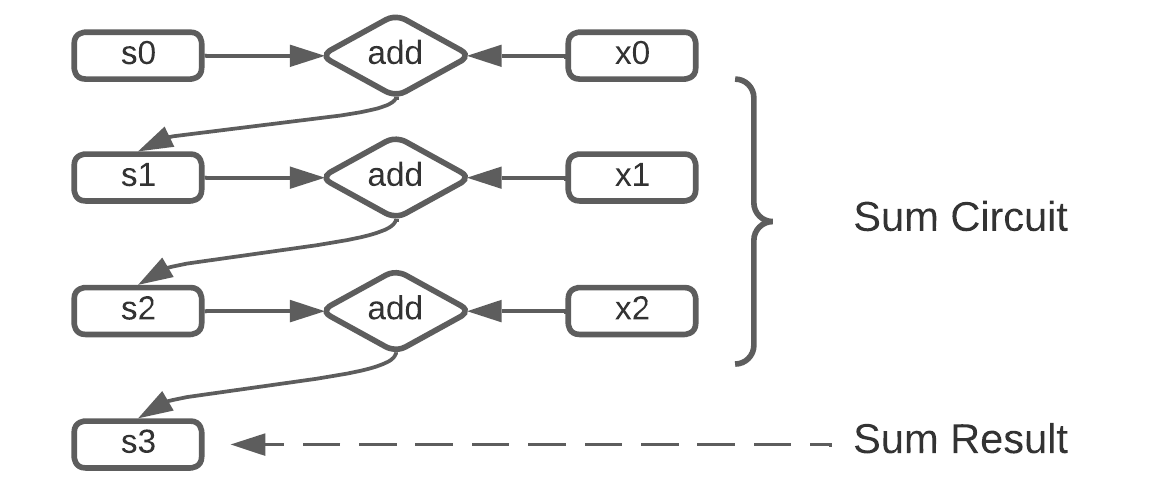
\includegraphics[scale=0.8]{figs/arithment-circuit.png}
}
\caption{Arithment Circuit of Sum}\label{fig:sum-gates}
\end{figure}

Now we have connected stateless programs to arithmetic circuits, and we know how to construct SNARKS of polynomial evaluation using PCS. Therefore it remains to establish a connection between arithmetic circuits with polynomials. This can be achieved by using interpolation techniques and copy constraints in PLONKish (see Section \ref{chp:constraint-system}).

%PCS 是polynomialbase的,constraint base ---> PCS
\subsection{Connecting Stateful Virtual Machine with Arithmetic Circuits}
\label{chp:encode-state-in-circuits}
Now we need to make a setup further. Instead of constructing a SNARK scheme for stateless programs, we would like to construct a SNARK scheme for a stateful virtual machine. We do not construct such SNARK from scratch; we construct it from the knowing ingredients which are the arithmetic circuits in Section \ref{chp:arith-circuits}. 

To start with, we establish the connection between a virtual machine and a program by treating the virtual machine as a program that generates a list of state transitions and each transition is defined as a monad function between states. We denote the transition function as $T_i$ which takes an input $s:State$ and outputs a new state $s':S$. The type of state $\mathcal{S}$ is defined as a tuple of \fullstate \, where $\mathcal{F}$ is the calling frame, $\mathcal{M}$ is the memory state, $\mathcal{S}_p$ is the stack and $\mathcal{I}$ is the image which contains code image $\mathcal{C}$ and initial memory $\mathcal{H}$.

Also for an instruction $op$ at address $addr$ in the image $\mathcal{I}$ of a WASM binary file, we define the transition semantic of $op$ to be a pair of $(t^{addr}_{op}, c^{addr}_{op})$ where $t^{address}_{op}$ is a state transition function and $c^{addr}_{op}$ is the control flow function from $S$ to the address of next instruction.

To define a valid sequence of transitions $T_i$, we first require that $T_0$ enforces the transition semantic of the instruction at the entry point $iaddr$ and for all $addr, s, k$, $T_k(s) = t^{iaddr}_{op}(s) \rightarrow T_{k+1} = t_{op'}^{iaddr'}$ where $iaddr' = c_{op}^{iaddr}(s)$ and $op'$ is the opcode of the instruction at $'iaddr$.

Second, with this setup we can map the execution of an executable image $I$ in a virtual machine $\mathcal{V}_m$ to a sequence of transition function $T_i$ over an initial state $s_0$. By denoting $s_i = T_i (T_{i-1}(\cdots T_0(s_0)))$ and $s_e$ to be the last state of the transition sequence, we require the final opcode of $T_{e}$ is returned and the depth of the calling frame of $s_e$ is zero $\mathcal{F}(s_e).depth = 0$.

We say a system of arithmetic circuits $C$ of transitions is equivalent to a WASM virtual machine if for any given entry point $iaddr_0$ there exists a unique sequence of $T_i$ satisfies $C$ and $T_0 = c^{iaddr_0}_{op}$.

%Stateless -> Statefull 的虚拟机:monadic function while s is hash
\subsection{Leverage zero-knowledge in ZKWASM}
A \zksnark\, is a SNARK scheme that provides a way for a prover to prove statements without leaking any information. When we construct the above SNARK scheme for a virtual machine in a zero-knowledge way, then we create a ZK Virtual machine that can prove the execution of certain program image without leaking any information.  This feature makes the ZK virtual machine extremely useful in scenarios where the prover would like to prove that certain output is calculated from the execution of a particular program image but does not want to leak the data used.
 
